\chapter*{Dodatak: Prikaz aktivnosti grupe}
		\addcontentsline{toc}{chapter}{Dodatak: Prikaz aktivnosti grupe}
		
		\section*{Dnevnik sastajanja}
		
		\textbf{\textit{Kontinuirano osvježavanje}}\\
		
		 \textit{U ovom dijelu potrebno je redovito osvježavati dnevnik sastajanja prema predlošku.}
		
		\begin{packed_enum}
			\item  sastanak
			
			\item[] \begin{packed_item}
				\item 20.10.2022., 13:45
				\item Prisustvovali: Laura Majer, Petra-Dunja Grujić-Ostojić, Fran Markulin, Karla Udiljak, Branimir Medvedec, Jura Starčević, Luka Radman, Marko Štrk
				\item Teme sastanka: 
				\begin{packed_item}
					\item  sastanak s asistenticom i demonstratoricom
					\item  raščišćavanje osnovnih dilema funkcionalnosti
					\item  analiza zadatka
				\end{packed_item}
			\end{packed_item}
			
			\item  sastanak
			\item[] \begin{packed_item}
				\item Datum: 02.11.2022., 13:00
				\item Prisustvovali: Fran Markulin, Karla Udiljak, Branimir Medvedec, Jura Starčević, Luka Radman, Marko Štrk
				\item Teme sastanka:
				\begin{packed_item}
					\item  podijela dužnosti:
					\begin{packed_item}
						\item  Fran Markulin: voditelj projekta, developer
						\item  Karla Udiljak: designer
						\item  Branimir Medvedec: developer
						\item  Jura Starčević: dokumentacija
						\item  Luka Radman: developer
						\item  Marko Štrk: dokumentacija
					\end{packed_item}
					\item  uvod u tehnologiju i arhitekturu koju bi koristili
					\item  rješavanje pitanja i nedoumica oko tehnologije i arhitekture
					\item  razrada strukture baze podataka
					\item  ostali dogovori
				\end{packed_item}
			\end{packed_item}

			\item  sastanak
			
			\item[] \begin{packed_item}
				\item 05.11.2022., 10:00
				\item Prisustvovali: Fran Markulin, Branimir Medvedec, Luka Radman
				\item Teme sastanka: 
				\begin{packed_item}
					\item  rad na razvoju aplikacije
				\end{packed_item}
			\end{packed_item}

			\item  sastanak
			
			\item[] \begin{packed_item}
				\item 13.11.2022., 15:00
				\item Prisustvovali: Fran Markulin, Karla Udiljak, Branimir Medvedec, Jura Starčević, Luka Radman, Marko Štrk
				\item Teme sastanka: 
				\begin{packed_item}
					\item  dokumentacija - što još treba i kako dokumentirati
					\item svaki član prezentirao svoj dio posla kako bi svi bili upoznati sa svime na projektu
					\item dogovoreni idući koraci
					\item podijela poslova
					\item zadani rokovi
				\end{packed_item}
			\end{packed_item}

			\item  sastanak
			
			\item[] \begin{packed_item}
				\item 15.11.2022, 7:30
				\item Prisustvovali: Fran Markulin, Branimir Medvedec, Luka Radman
				\item Teme sastanka: 
				\begin{packed_item}
					\item  rad na razvoju aplikacije
					\item priprema za prvu predaju
				\end{packed_item}
			\end{packed_item}

			\item  sastanak
			
			\item[] \begin{packed_item}
				\item 16.11.2022., 10:30
				\item Prisustvovali: Fran Markulin, Branimir Medvedec
				\item Teme sastanka: 
				\begin{packed_item}
					\item  komentiranje programskog koda
					\item rad na dokumentaciji
					\item priprema za izradu dijagrama razreda
				\end{packed_item}
			\end{packed_item}
			
			%
			
		\end{packed_enum}
		
		\eject
		\section*{Tablica aktivnosti}
		
			%\textbf{\textit{Kontinuirano osvježavanje}}\\
			
			% \textit{Napomena: Doprinose u aktivnostima treba navesti u satima po članovima grupe po aktivnosti.}

			\begin{longtblr}[
					label=none,
				]{
					vlines,hlines,
					width = \textwidth,
					colspec={X[6, l]X[1, c]X[1, c]X[1, c]X[1, c]X[1, c]X[1, c]}, 
					vline{1} = {1}{text=\clap{}},
					hline{1} = {1}{text=\clap{}},
					rowhead = 1,
				} 
				\multicolumn{1}{c|}{} & \multicolumn{1}{c|}{\rotatebox{90}{\textbf{Fran Markulin}}} & \multicolumn{1}{c|}{\rotatebox{90}{\textbf{Branimir Medvedec}}} &	\multicolumn{1}{c|}{\rotatebox{90}{\textbf{Luka Radman}}} & \multicolumn{1}{c|}{\rotatebox{90}{\textbf{Karla Udiljak }}} &	\multicolumn{1}{c|}{\rotatebox{90}{\textbf{ Jura Starčević}}} & \multicolumn{1}{c|}{\rotatebox{90}{\textbf{Marko Štrk }}}  \\  
				Upravljanje projektom 		&24  &  &  &  &  &   \\ 
				Opis projektnog zadatka 	&  &  &  &  &6  &   \\ 
				
				Funkcionalni zahtjevi       & 1 &  &  & 1 &1.5  &    \\ 
				Opis pojedinih obrazaca 	&  &  &  &  &  &  4  \\ 
				Dijagram obrazaca 			&  &  &  & 4 &  &    \\ 
				Sekvencijski dijagrami 		&  &  &  &6  &  &    \\ 
				Opis ostalih zahtjeva 		&  &  &  &  &  & 0.5  \\ 

				Arhitektura i dizajn sustava	 &3  &  &  &  & 1.5  &    \\ 
				Baza podataka				&1  &  &  &  & 3 &    \\ 
				Dijagram razreda 			&4  &  & 2 &  &  &  1  \\ 
				%Dijagram stanja				&  &  &  &  &  &   \\ 
				%Dijagram aktivnosti 		&  &  &  &  &  &    \\ 
				%Dijagram komponenti			&  &  &  &  &  &    \\ 
				%Korištene tehnologije i alati 		&  &  &  &  &  &    \\ 
				%Ispitivanje programskog rješenja 	&  &  &  &  &  &   \\ 
				%Dijagram razmještaja			&  &  &  &  &  &    \\ 
				%Upute za puštanje u pogon 		&  &  &  &  &  &   \\  
				%Zaključak i budući rad 		&  &  &  &  &  &    \\  
				Popis literature 			& 0.5 &  &  &  &1  &   \\  
                Izrada login stranice			& 2 & 8 &  &  &  &   \\
                Izrada register stranice			& 2 & 6 & 5 &  &  &   \\
                Izrada komponente VlasnikForm			& 3 & 6 & 6 &  &  &   \\
                Izrada komponente PrivatnaForm			& 3 & 4 & 3 &  &  &   \\
                Izrada user info stranice			& 2 & 4 & 8 &  &  &   \\
                Izrada komunikacije s bazom podataka			& 6 &  &  &  &  &   \\
                Izrada konteksta			& 2 &  &  &  &  &   \\
                Izrada komponente layout			& 1 &  &  &  &  &   \\
                Izrada posebnih funkcija (hook.js)  & 1 &  &  &  &  &   \\
                Izrada baze podataka  & 4 &  &1  &  &  &   \\
                Izrada baze podataka  & 2 &  &  &  &  &   \\
                Vođenje git repotizorija & 5 &  &  &  &  &   \\
                Design &  &  &  & 16 &  &   \\
                Dnevnik sastajanja & 1 &  &  &  &0.5  &   \\
                Moderiranje Latex dokumenta & 1 &  &  &  &25  & 2  \\
                
	\end{longtblr}

	
					
					
		\eject
		\section*{Dijagrami pregleda promjena}
		\begin{figure}[H]
			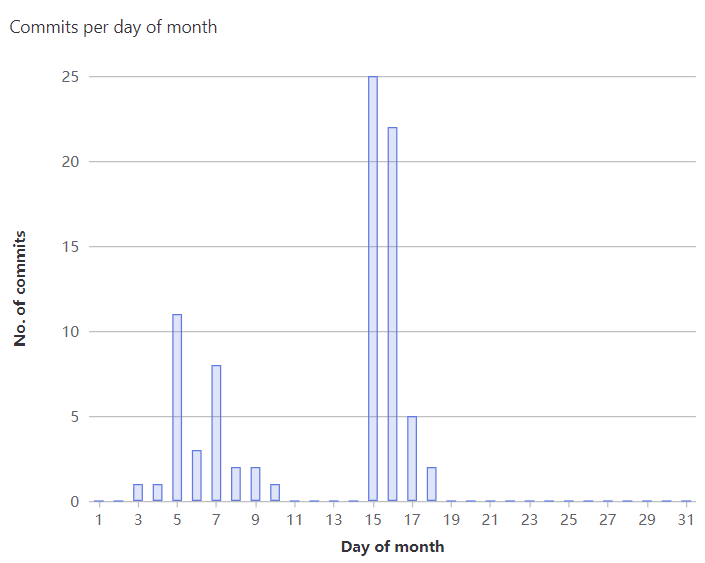
\includegraphics[scale=0.7]{slike/Aktivnost.png}
			\centering
			\caption{Dijagram baze podataka}
			\label{fig:promjene}
		          \end{figure}
		%\textbf{\textit{dio 2. revizije}}\\
		
		%\textit{Prenijeti dijagram pregleda promjena nad datotekama projekta. Potrebno je na kraju projekta generirane grafove s gitlaba prenijeti u ovo poglavlje dokumentacije. Dijagrami za vlastiti projekt se mogu preuzeti s gitlab.com stranice, u izborniku Repository, pritiskom na stavku Contributors.}
		
	